%\documentclass[]{article}
\documentclass[]{elsarticle}
\usepackage{amsmath}
%\usepackage{cite}
\usepackage{bm}
\usepackage{color}
\usepackage{amssymb}
\usepackage{graphicx}
\usepackage{epstopdf}
%\usepackage[margin=1in]{geometry}
\usepackage{caption}
\usepackage{subcaption}
\usepackage{multirow}
\usepackage{color}
\usepackage{xcolor}
\usepackage[final]{pdfpages}
\usepackage{lineno}
\modulolinenumbers[5]

%%%so that figures appear in their section
\usepackage[section]{placeins}

\begin{document}


\linenumbers

\section*{Introduction}
The textwidht for this paper is : \the\textwidth


To compile the code
\begin{verbatim}
cmake .
make
\end{verbatim}

To generate the measurements
\begin{verbatim}
./data gcase00.cfg
\end{verbatim}

To run the static parameter case
\begin{verbatim}
mpirun -np 12 ./run case00.cfg
\end{verbatim}


To run the time-varying parameter case
\begin{verbatim}
mpirun -np 10 ./run case00b.cfg
mpirun -np 10 ./run case00c.cfg
mpirun -np 10 ./run case00d.cfg
mpirun -np 10 ./run case00e.cfg
mpirun -np 10 ./run case00f.cfg
\end{verbatim}
To display the results (eps figures will be saved in the figs folder)
\begin{verbatim}
python draw.py
\end{verbatim}

\subsection*{Configuration files}
The various parameters can be changed in different files.
In the file "functions.cpp", the models are coded. In the ".cfg" files, the parameters for each cases are present. The file "gcase00.cfg" controls data generation. The important parameters are
\begin{verbatim}
	name 			= 	"First Order SDE (colored noise!)";
	handle 			=	"FirstOrder";
	folder			=	"Case00";
	initialState 	=	[1.0];
	parameters			=	[1.0, 0.01];
	time			=	10.0;
	dt				=	0.001;
	stepsBetweenMeasurements = 10;
	NSR				=	0.25;
\end{verbatim}
where handle corresponds to the function in "functions.cpp". The {\bf folder} "Case00" is where the measurements will be stored. The initial state of the system is $x = 1.0$ ( {\bf initialState}). The parameter vector $[1.0, 0.01]$ corresponds to $[\alpha, \sigma]$. The keyword {\bf time} controls for how long is the system simulated, {\bf dt} is the timestep, {\bf stepsBetweenMeasurements} controls how many time steps between each measurements and {\bf NSR} is the noise to signal ratio.

The other configuration files control the parameter and state estimation problem. In "case00.cfg" the following can be found
\begin{verbatim}
folder																=	"Case00";
dt																		=	0.001;
fStepsBetweenMeasurements 						=	10;
measurementCov												=	"variance.dat";
data																	=	"data.dat";
Parameter_Estimation 									= true;
Evidence_Estimation 									= false;
State_Estimation											= false;
seruns 																= 1;
\end{verbatim}
Where {\bf folder} specifies where the measurements can bve found, {\bf data} and { \bf measurementCov} are the name of the files where measurements and the measurement variance are stored.  The true and false indicates that parameter estimation is performed but stand alone state estimation is not performed. The state estimation procedure included in the parameter estimation problem is still performed. For each proposed models we have the following configuration keywords

\begin{verbatim}
	run							=	true;
	name 						=	"StaticParameters";
	state_estimator				=	"ekf";
	handle 						=	"m2";
	initialState 				=	[5.0];
	nprocs						= 1;
	initialStateVariance 		= ([0.1])
	//parameters 				= (0.2, 0.1);
	prior					= 	(
		"Uniform", 0.0, 10.0,
		"Uniform", 0.0, 10.0
	);
	parallelGroups				= 8;
	MCMC_CONFIG						=	{
		Method = "TMCMC";
		dim = 2;
		window = 40000;
		};
\end{verbatim}

{\bf run} controls wether this model will be run of not. The keyword {\bf state\_estimator} controls what filter is used for state estimation. The {\bf handle} links to the statespace created in "functions.cpp". {\bf initialState} and {\bf initialStateVariance} are the initial mean and covariance of the state. We use TMCMC to sample the posterior distribution. The dimension of the pdf is {\bf dim} $=2$ and there are window samples divided into 8 {\bf parallelGroups}. Each core is responsible for a group. {\bf nprocs} and {\bf parameters} are not used here.


The other configuration files control the state estimation procedure when the state is augmented. There could only be one configuration file but they are separated for convenience. For example, in case00d.cfg the following can be found
\begin{verbatim}
	run										= true;
	name 									=	"TimeVaryingParametersEnkfD";
	state_estimator				=	"enkfmpi";
	handle 								=	"m1enkf";
	initialState 					=	[1.0, 5.0];
	nparticles							=	10000;
	nprocs								=	4;
	initialStateVariance 	= ([0.1, 0.0],[0.0, 0.000001])
	parameters 						= (0.01,0.01);
\end{verbatim}
The statespace used is m1enkf defined in functions.cpp. The filter used is the parallel Enkf ({\bf state\_estimator} = "enkfmpi") the initial state is controlled by {\bf initialState}. The filter uses 4 processsors ({\bf nprocs}) and is composed of 10000 particles ({\bf nparticles}). The initial state variance ({\bf initialStateVariance}) is 
\begin{equation}
P_0 = \begin{bmatrix}
0.1 & 0 \\
0 & 0.000001
\end{bmatrix}
\end{equation}
and the parameters for $[\sigma, \gamma]$ are defined by {\bf parameters}. These can be changed as well.

\section*{Description of the system}

Consider the following linear system
\begin{equation}
\dot{x} + a x = \sigma W(t)
\end{equation}
with available measurements described by
\begin{equation}
d_k = x_k + \varepsilon_k
\end{equation}
where $\varepsilon_k$ is a GRV with zero mean and a variance chosen so that the noise to signal ratio is $0.25$. The discrete representation of this system is given by
\begin{equation}
x_{k+1} = (1.0 - a \Delta t) x_k + \sigma \sqrt{\Delta t} q_k
\end{equation}
where $q_k$ is drawn from a zero mean and unit variance Gaussian distribution. A realization of this system is generated with a initial condition of $x(0) = 1.0$. Noisy measurements are generated. The measurements are kept dense to insure that the estimation of the time-varying parameter $a$ will succeed with EKF.

\begin{figure}[!htb]
\centering
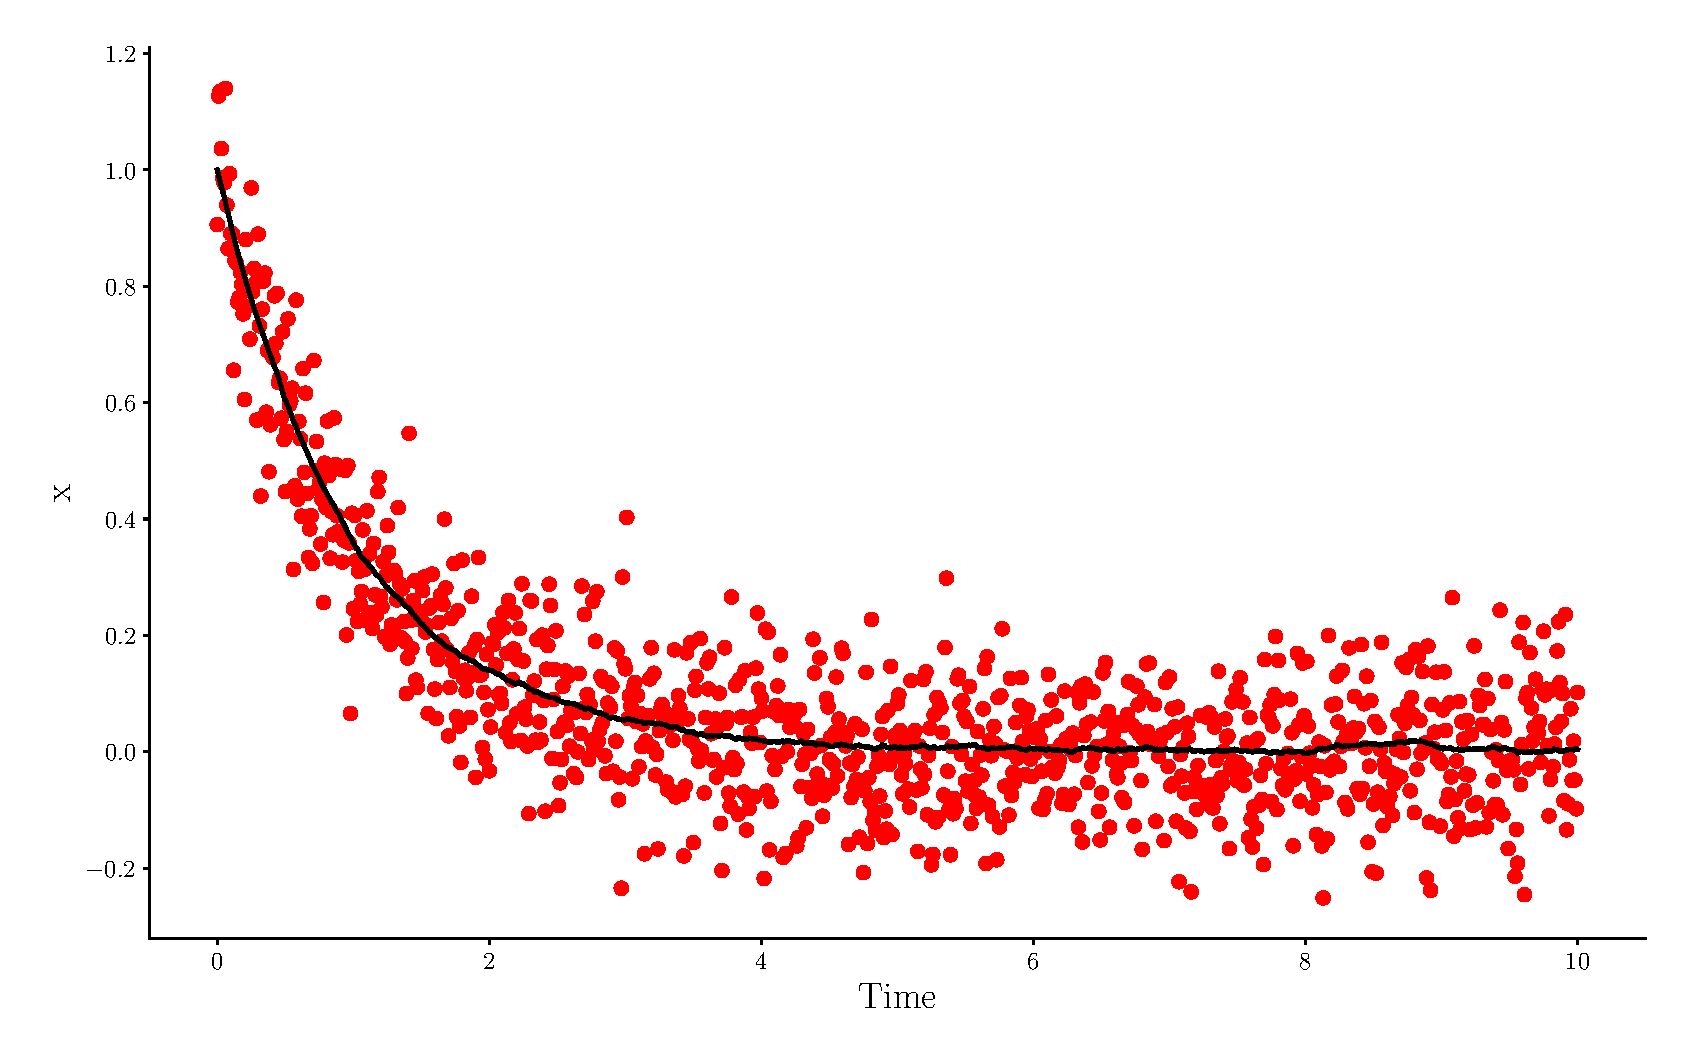
\includegraphics[width=\linewidth,keepaspectratio]{./figs/case00_data.eps}
\caption{Synthetic measurements}
\label{fig:data}
\end{figure}


The are two approaches considered here to estimate the unknown parameter $a$. The first method, $a$ is treated as a static parameter. In this approach, both $a$ and $\sigma$ are estimated.

\section*{Static parameter}

An MCMC algorithm is used to sample from the parameter posterior distribution. In the first case, only the static parameter $a$ is estimated. The marginal pdf of parameter $a$ is shown in Fig.~\ref{fig:aOnly}. In the second scenario both $a$ and $\sigma$ are estimated. The marginal pdfs are shown in Fig.~\ref{fig:a} and Fig.~\ref{fig:sigma}.

\begin{figure}[!htb]
\centering
\includegraphics[width=\linewidth,keepaspectratio]{./figs/case00_aOnly.eps}
\caption{Pdf of static parameter a when it is the only unknown. True value of $a$ is $1.0$}
\label{fig:aOnly}
\end{figure}

\begin{figure}[!htb]
\centering
\includegraphics[width=\linewidth,keepaspectratio]{./figs/case00_a.eps}
\caption{Marginal pdf of static parameter a. True value of $a$ is $1.0$}
\label{fig:a}
\end{figure}

\begin{figure}[!htb]
\centering
\includegraphics[width=\linewidth,keepaspectratio]{./figs/case00_sigma.eps}
\caption{Marginal pdf of static parameter $\sigma$. True value of $\sigma$ is $0.01$.}
\label{fig:sigma}
\end{figure}

\section*{Time-varying parameter}
In the second approach, $a$ is treated as a time-varying parameter. The state of the system, fully described by $x$ is augmented with $a_k$. The original static parameter $a$ is now varying. In the first method, a MCMC algorithm was used to estimate the posterior pdf of the parameters, in the second method, only state estimation is performed. This approach is less expensive, however augmenting the state with the parameters makes the problem nonlinear. State estimation will be performed using EKF, EnKF and PF. The modified discrete system for the first scenario is described by 

\begin{align}
x_{k+1} &= (1.0 - a_k \Delta t) x_k + \sigma \sqrt{\Delta t} w_k \\ 
a_{k+1} &= a_k + \gamma \sqrt{\Delta t} q_k
\end{align}
where $\gamma$ is a tuning parameter. This value can be seen as a parameter controlling how much the parameter $a$ is allowed to change during the forecast. The strength of the noise is assumed known with $\sigma = 0.01$. The estimate of $a_k$ is updated with available measurements. State estimation is performed using three different filters, EKF, EnKF and PF. Nonlinear filters are necessary due the nonlinear nature of the augmented system. The estimate of $x$ and $a$ are shown in the following figures. The intial variance of the state is set to 
\begin{equation}
P_0 = \begin{bmatrix}
0.1 & 0 \\
0 & 0.1
\end{bmatrix}
\end{equation}
The effect of the initial variance is not studied in this work. But there might be an impact on the quality of the estimates when bad intial estimates are provided.
The state estimage of $x$ and $a$ are shown in Fig.~\ref{fig:x1} and Fig.~\ref{fig:a1}. In this case the initial conditions are $[1.0, 1.2]$. The noise parameters are $\sigma = 0.01$ and $\gamma = 0.01$.

\begin{figure}[!hptb]
\centering
\includegraphics[width=\linewidth,keepaspectratio]{./figs/case00_x_estimate.eps}
\caption{Mean estimate of x when $a=1.2$.}
\label{fig:x1}
\end{figure}

\begin{figure}[!hptb]
\centering
\includegraphics[width=\linewidth,keepaspectratio]{./figs/case00_a_estimate.eps}
\caption{Mean estimate of a when $a=1.2$.}
\label{fig:a1}
\end{figure}

The red dashed lines correspond to $99\%$ bounds of the EKF estimate.

\subsection*{Effect of initial conditions}

In this section, the value of the initial state variance, the noise strenght and the initial estimate of $a$ are changed. The different cases are outlined in Table~\ref{table:1}. 
\begin{table}[]
\centering
\caption{Overview of cases}
\label{table:1}
\begin{tabular}{|l|lll|l|}
\hline
Cases  & $a_0$  & $Var(a_0)$  & $\gamma$ & Figures \\
\hline
Case 1 & $5.0$ & $0.1$  & $0.01$ & 7,8 \\
Case 2 & $5.0$ & $0.000001$ & $0.01$ & 9,10 \\
Case 3 & $5.0$ & $0.000001$ & $2.0$ & 11,12\\
Case 4 & $5.0$ & $2.0$  &   $0.000001$ & 13,14\\
\hline
\end{tabular}
\end{table}

Performing state estimation by augmenting the state provides the following estimates shown in Fig.~\ref{fig:x2} and Fig.~\ref{fig:a2}. In this case the initial conditions are $[1.0, 5.0]$. The variance of $a_0$ is $0.1$ and the value of $\gamma$ is $0.01$. In this scenario PF doesn't perform adequately and I do not know why. I've increased the number of particles to 100 000 (about 10 times the number of particles used by EnKF) and still have the same result. I will need to investigate why it doesn't perform as it should. I think part of the reason is that the initial variance for $a_0$ is to restrictive, it may be that in the update phase no particles have a high loglikelihoood and thus we are running into numerical problems where the weights are too small.


\begin{figure}[!htb]
\centering
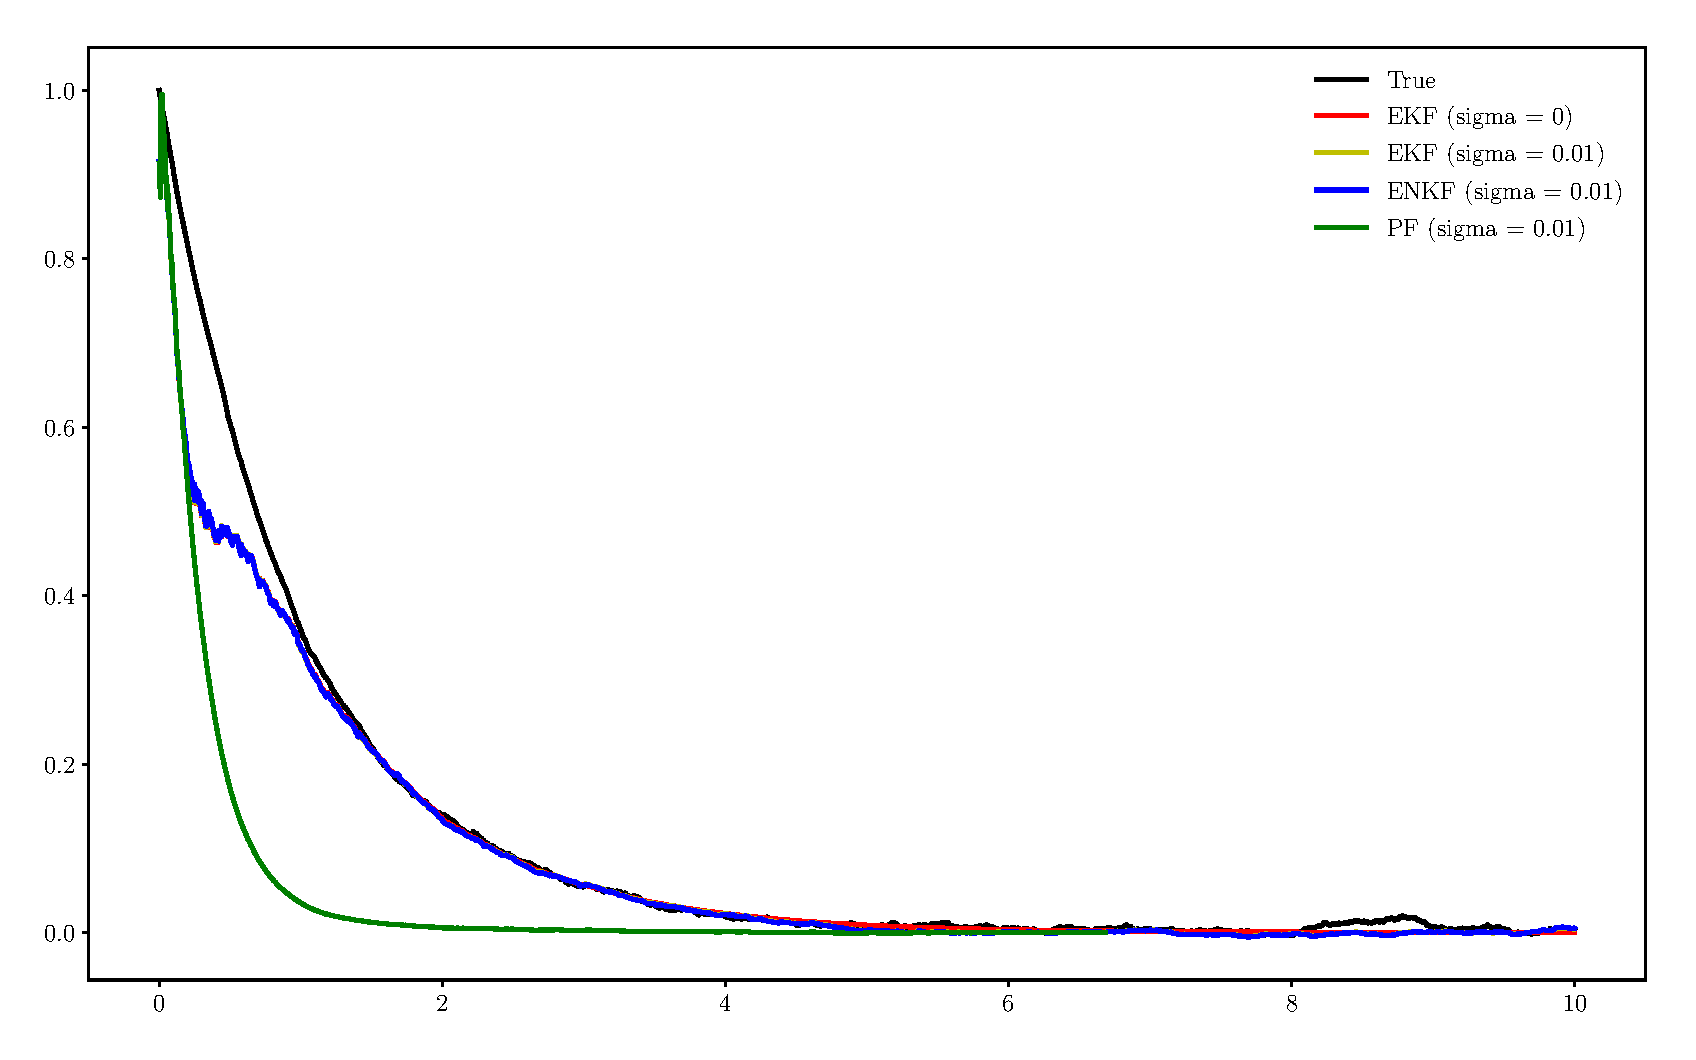
\includegraphics[width=\linewidth,keepaspectratio]{./figs/case00_x_estimate2.eps}
\caption{(Case 1) Mean estimate of x.}
\label{fig:x2}
\end{figure}

\begin{figure}[!htb]
\centering
\includegraphics[width=\linewidth,keepaspectratio]{./figs/case00_a_estimate2.eps}
\caption{(Case 1) Mean estimate of a.}
\label{fig:a2}
\end{figure}
 
The results of state estimation for Case 2 are shown in Fig.~\ref{fig:x3} and Fig.~\ref{fig:a3}. The initial variance of $a_0$ is significantly decreased. The value of $a$ doesn't change and can't be updated by incoming measurements due to the restrictive nature of the initial condition and the small $\gamma$.

\begin{figure}[!htb]
\centering
\includegraphics[width=\linewidth,keepaspectratio]{./figs/case00_x_estimate3.eps}
\caption{(Case 2) Mean estimate of x.}
\label{fig:x3}
\end{figure}

\begin{figure}[!htb]
\centering
\includegraphics[width=\linewidth,keepaspectratio]{./figs/case00_a_estimate3.eps}
\caption{(Case 2) Mean estimate of a.}
\label{fig:a3}
\end{figure}


The results of state estimation for Case 3 are shown in Fig.~\ref{fig:x4} and Fig.~\ref{fig:a4}. The initial variance of $a_0$ is the same as the previous case, but the value of $\gamma$ is significantly higher. The mean value of $a$ changes but it can't converge to a specific value. 


\begin{figure}[!htb]
\centering
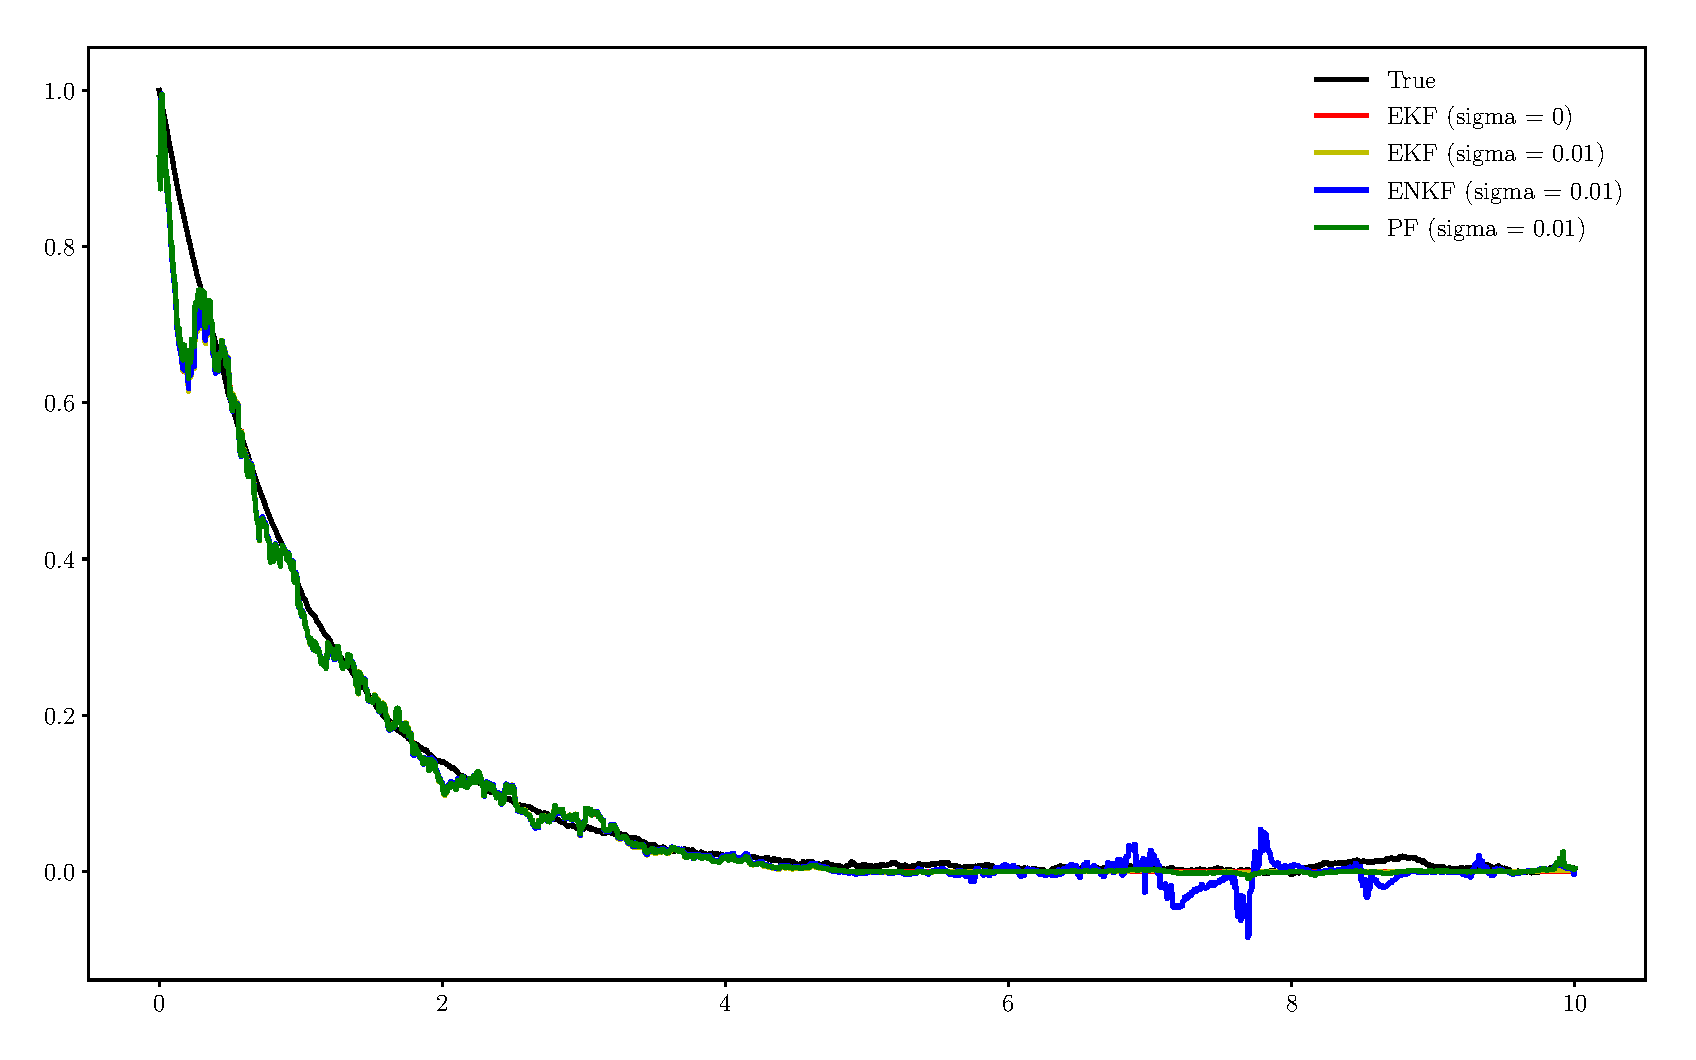
\includegraphics[width=\linewidth,keepaspectratio]{./figs/case00_x_estimate4.eps}
\caption{(Case 3) Mean estimate of x.}
\label{fig:x4}
\end{figure}

\begin{figure}[!htb]
\centering
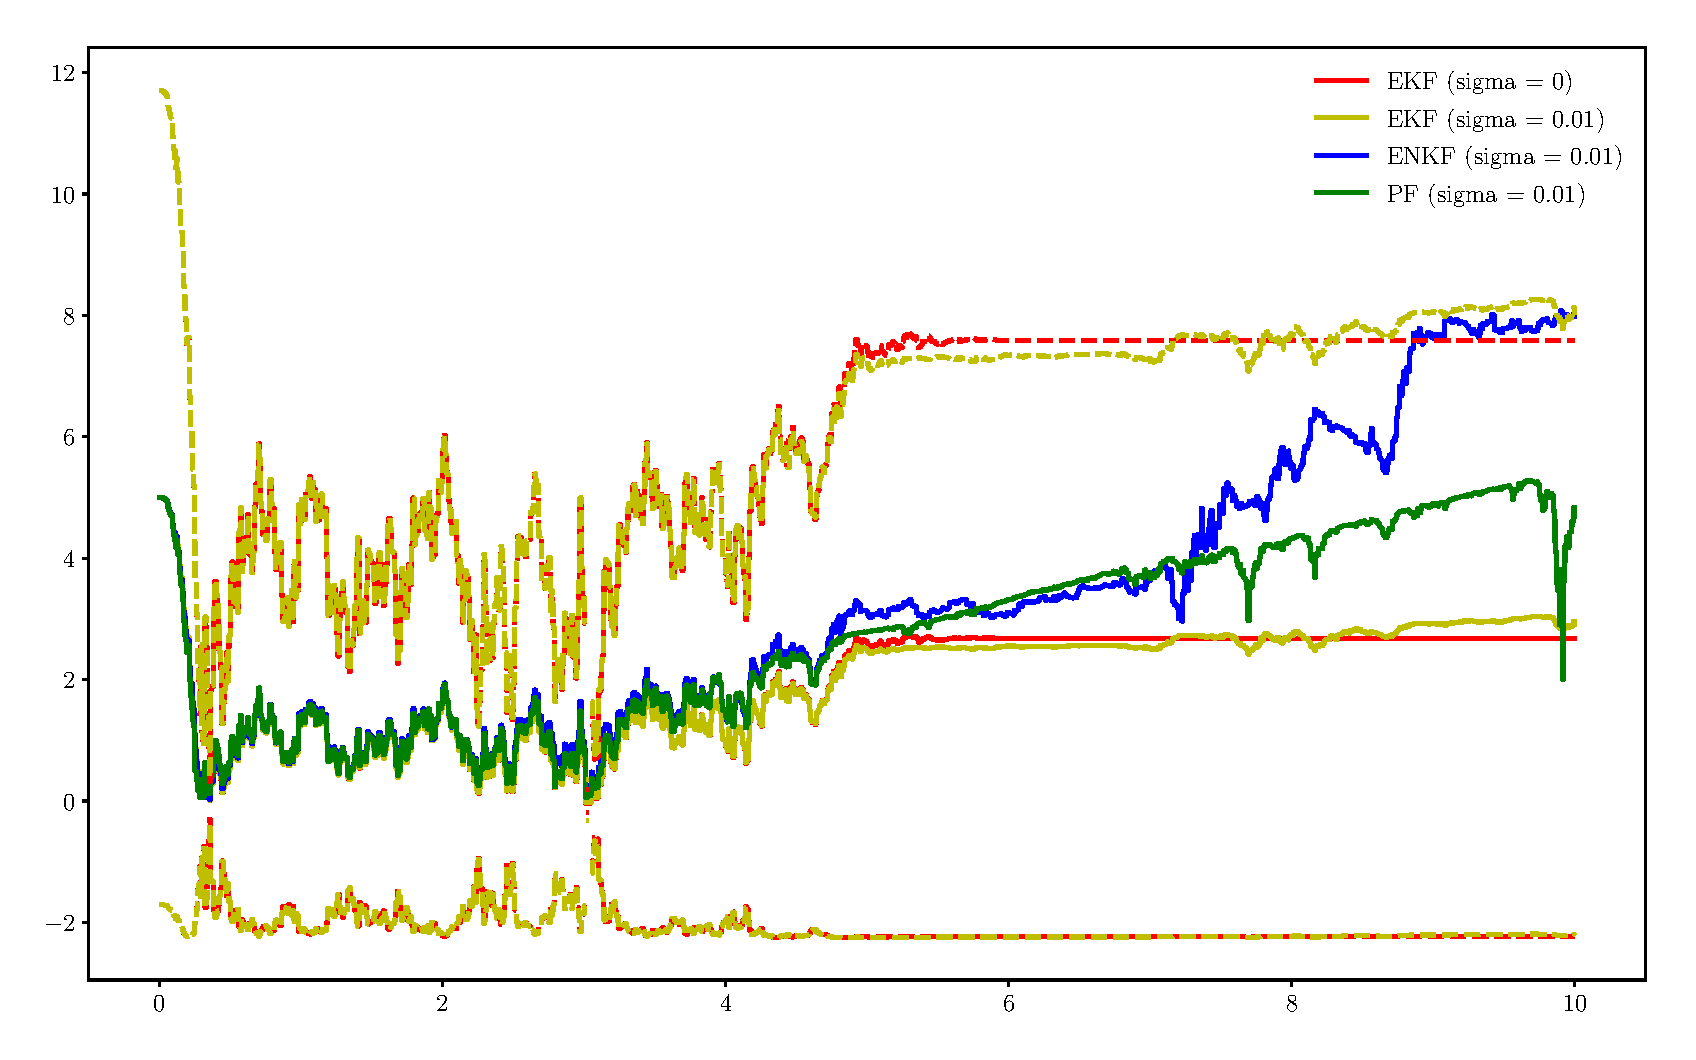
\includegraphics[width=\linewidth,keepaspectratio]{./figs/case00_a_estimate4.eps}
\caption{(Case 3) Mean estimate of a.}
\label{fig:a4}
\end{figure}

The results of state estimation for Case 4 are shown in Fig.~\ref{fig:x5} and Fig.~\ref{fig:a5}. The initial variance of $a_0$ is significantly larger and we have a smaller value of $\gamma$. The results are satisfactory because the of larger variance of $a$. In that case the true value lies in a high probability region of the prior. The effect of $\gamma$ is not needed.

\begin{figure}[!htb]
\centering
\includegraphics[width=\linewidth,keepaspectratio]{./figs/case00_x_estimate5.eps}
\caption{(Case 4) Mean estimate of x.}
\label{fig:x5}
\end{figure}

\begin{figure}[!htb]
\centering
\includegraphics[width=\linewidth,keepaspectratio]{./figs/case00_a_estimate5.eps}
\caption{(Case 4) Mean estimate of a.}
\label{fig:a5}
\end{figure}

\end{document}
